\chapter{Séance 1: lundi 26 novembre 2018}

\section{Exemple introductif I:\ L'Exécution}
\label{sec:exemple-intr-i}

On considère deux variables aléatoires \(X\) et \(Y\) à valeurs dans
\(\left\{ 0,1 \right\}\), qui représentent un tireur qui tire (\(X=1\)) ou
non (\(X=0\)) et un condamné qui meurt (\(Y=1\)) ou non (\(Y=0\)). On
suppose que les variables \((X,Y)\) suivent une distribution jointe \(P\) qui est
telle que \(X=Y=1\) avec probabilité \(1/2\) et \(X=Y=0\) avec probabilité
\(1/2\): \[ P\left( X=1,\ Y=1 \right)=P(X=0,Y=0)=\frac{1}{2}. \] Les
configurations \((X=0,Y=1)\) et \((X=1,Y=0)\) sont donc de probabilité
nulle.  Par ailleurs, \emph{on sait} que c'est \(X=1\) (le tir) qui \emph{cause}
\(Y=1\) (la mort), en un sens qui reste à préciser; on en a en tout cas
l'intuition.
\begin{center}
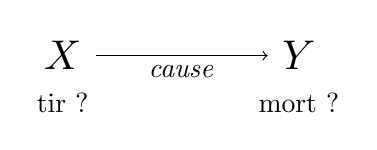
\begin{tikzpicture}
\node[scale=1.5] (X) at (0,0) {$X$};
\node[scale=1.5] (Y) at (3,0) {$Y$};
\draw[->] (X) node[below=10pt]{tir ?} -- node[midway,below]{\emph{\og cause\fg}} (Y)node[below=10pt]{mort ?};
\end{tikzpicture}
\end{center}

\begin{remark}
La distribution $P$ est symétrique en $X$ et $Y$. Ce n'est pas le cas du lien de causalité. 
On voit donc que l'information du lien de causalité ne peut pas être contenue dans la distribution $P$.
Les liens de causalité sont des informations qui viennent en supplément (pour ainsi dire) de la distribution $P$.
\end{remark}

Il y a au moins deux types de démarches qu'on peut imaginer:
\begin{itemize}
\item soit on cherche à déterminer des liens de causalité qu'on ne connaît pas;
\item soit on connaît les liens de causalité, et on souhaite les utiliser
pour répondre à des questions.
\end{itemize}
Dans un premier temps, on va se pencher sur la deuxième démarche
ci-dessus. Les liens de causalité seront donc une \emph{connaissance} (un
\emph{prior knowledge}) dont nous disposons.

\textbf{Question}: Que signifie au juste \og\(X=1\) cause \(Y=1\)\fg \ldots{} ?

\textbf{Réponse}: Cela signifique que:
\begin{itemize}
\item si l'on intervient pour forcer \(X=1\) (on force le tireur à tirer),
alors \(Y=1\) (le condamné meurt) avec probabilité \(1\);
\item en revanche, si l'on intervient pour forcer \(Y=1\) (on intervient
pour tuer le condamné, en le poignardant par exemple), alors cela
n'affectera pas le tireur: on aura toujours \(X=1\) avec probabilité seulement \(1/2\).
\end{itemize}
Un lien de causalité est donc une affirmation qui porte sur les
effets d'une \emph{intervention} (qui modifie donc le phénomène étudié).

On va voir que la donnée d'une distribution jointe initiale \(P\), de liens de
causalité connus, et d'une \emph{intervention} (par exemple \(X=x\)) qu'on considère,
définit une distribution jointe modifié, que l'on va noter \(P_{X=x}=P(\,\cdot\,|\,do(X=x))\).
Gardons à l'esprit le schéma suivant.
\[ \text{\parbox{2cm}{\centering distribution jointe initiale
$P$}}+\parbox{2cm}{\centering liens de causalité}+
\parbox{2cm}{\centering intervention $X=x$}=\parbox{4cm}{\centering
distribution modifiée $P_{X=x}$}  \]

\section{Exemple introductif II:\ Le Sol mouillé}
\label{sec:exemple-intr-ii}

On considère ici quatre variables \(X_1,\dots,X_4\) à valeurs dans \(\left\{ 0,1 \right\}\).
\begin{itemize}
\item \(X_1\) représente la saison qui peut être dans deux états différents: saison pluvieuse (\(X_1=1\)) et saison non-pluvieuse (\(X_1=0\)).
\item \(X_2\) représente la météo actuelle: s'il pleut (\(X_2=1\)) ou s'il ne pleut pas (\(X_2=0\)).
\item \(X_3\) représente l'état d'un arroseur automatique: s'il est allumé
(\(X_3=1\)) ou éteint (\(X_3=0\)).
\item \(X_4\) représente l'état du sol: s'il est mouillé (\(X_4=1\)) ou non (\(X_4=0\)).
\end{itemize}
La distribution jointe \(P\) des variables \((X_1,\dots,X_4)\) est définie
de la manière suivante.
\begin{itemize}
\item La saison est pluvieuse avec probabilité \(1/2\):
\[ P(X_1=1)=\frac{1}{2}.  \]
\item Si la saison est pluvieuse, il pleut avec probabilité \(3/4\), et si
la saison n'est pas pluvieuse, il pleut avec probabilité \(1/4\):
\begin{align*}
P\left( X_2=1\,\middle|\,X_1=1 \right)&=\frac{3}{4}\\
P\left( X_2=1\,\middle|\,X_1=0 \right)&=\frac{1}{4}.
\end{align*}
\item L'arroseur automatique est éteint en saison pluvieuse, et allumé en
saison non pluvieuse; \(X_3\) est donc une fonction déterministe de
\(X_1\):
\[ X_3=1-X_1. \]
\item Le sol et mouillé s'il pleut et/ou si l'arroseur auomatique est
allumé; \(X_4\) est donc une fonction déterministe de \(X_2\) et \(X_3\):
\[ X_4=\max_{}(X_2,X_3). \]
\end{itemize}
Par ailleurs, notre intuition nous donne les liens de causalité que
l'on représente de la façon suivante.
\begin{center}
\begin{tikzpicture}[scale=2]
\node[scale=1.5] (X1) at (0,2) {$X_1$};
\node[scale=1.5] (X2) at (1,1) {$X_2$};
\node[scale=1.5] (X3) at (-1,1) {$X_3$};
\node[scale=1.5] (X4) at (0,0) {$X_4$};
\draw[->] (X1) node[above=10pt]{saison pluvieuse ?} -- (X2);
\draw[->] (X2) node[right=15pt]{pluie ?} -- (X4) node[below=10pt]{sol mouillé ?};
\draw[->] (X1) -- (X3) node[left=10pt]{arroseur ?};
\draw[->] (X3) -- (X4);
\end{tikzpicture}
\end{center}
On peut se demander pourquoi on n'a pas mis de flèche de \(X_1\) vers
\(X_4\) alors que la saison influence clairement (au sens de la
causalité) l'état du sol. Il se trouve qu'il est tout à fait correct
d'ajouter la flèche \(X_1\to X_4\), mais on verra ci-dessous que moins on
met de flèche, et plus on a d'informations, car c'est en fait
l'\emph{absence de flèche} qui est porteuse d'information. En l'occurence, on
a pu ne pas mettre la flèche \(X_1\to X_4\) car même s'il existe
un lien de causalité (\emph{indirect}) de \(X_1\) vers \(X_4\), la connaissance
des valeurs \(X_2\) et de \(X_3\) déterminent entièrement la loi de
\(X_4\). Ces idées seront précisées et formalisées plus bas.

On va à présent utiliser la distribution \(P\) ainsi que liens de
causalité qu'on s'est donné pour répondre à la question suivante.

\textbf{Question}: Quelle est la probabilité d'avoir le sol sec si on \emph{force}
 l'arrosage automatique à être éteint? Autrement dit, quelle est la
 valeur de
 \[ P_{X_3=0}(X_4=1)\quad ? \]

\textbf{Solution \emph{informelle}}: Puisqu'on \emph{force} ici l'arronsage
 automatique à être éteint (\(X_3=0\)), le sol est mouillé si et
 seulement s'il pleut (\(X_2=1\)). On a sous-entendu ici que la
 la variable \(X_4\) est affectée par l'intervention \(X_3=0\) (c'est
 ainsi qu'il convient d'interpréter la flèche \(X_3\to X_4\)). Donc: 
 \[ P_{X_3=0}(X_4=1)=P_{X_3=0}(X_2=1). \]
 En revanche, il n'y a pas de chemin fléché allant de \(X_3\) à \(X_2\),
 donc la loi de \(X_2\) reste inchangée par l'intervention \(X_3=0\), donc:
 \[ P_{X_3=0}(X_2=1)=P(X_2=1)=\frac{1}{2}. \]
 Donc, la réponse à la question est \(1/2\).

On peut se demander si cela ne revient pas tout simplement à
considérer l'\emph{espérance conditionnelle} sachant $X_3=0$. On va voir que non; montrons que:
\[ P_{X_3=0}(X_4=1)\neq P(X_4=1|X_3=0). \]
On sait que l'évènement \(X_3=0\) est
le même que \(X_1=1\) (car \(X_3=1-X_1\)).
Par ailleurs, si on conditionne par \(X_3=0\), l'évènement \(X_4=1\) est
le même que \(X_2=1\) (car \(X_4=\max_{}(X_2,X_3)\)).
Ainsi, on peut écrire:
\begin{align*}
P(X_4=1|X_3=0)&=P(X_2=1|X_3=0)\\
&=P(X_2=1|X_1=1)\\
&=\frac{3}{4}.
\end{align*}
La distribution qui résulte de l'intervention $X_3=0$ n'est donc pas
la même que l'espérance conditionnelle sachant $X_3=0$.

\section{Notations et conventions}
\label{sec:notat-et-conv}

On tâchera de suivre au plus près les notations du livre de Pearl \cite{pearl2009causality} tout
en renforçant un peu la rigueur du formalisme.
\begin{itemize}
\item Dans la suite, \(V=(X_i)_{i\in I}\) ou \(V=(V_i)_{i\in I}\) sera une
famille \emph{finie} de variables aléatoires.
\item Si \(V=(V_i)_{i\in I}\), on dit (par abus de langage) que:
\begin{itemize}
\item la variable \(X\) \emph{appartient} à \(V\) s'il existe \(i\in I\) tel que \(X=V_i\). On note
alors \(X\in V\).
\item \(X\) est un \emph{sous-ensemble} de \(V\) si \(X=(V_i)_{i\in J}\) avec
\(J\subset I\). On note alors \(X\subset V\).
\end{itemize}
\item On suppose que l'ensemble des valeurs prises par une des
  variables aléatoires est \emph{fini}.
\item Pour \(X\in V\) ou \(X\subset V\), on note \(D_X\) l'ensemble (fini donc)
des valeurs prises par \(X\).
\item Typiquement, on notera \(x\in D_X\) une valeur possible pour \(X\)
(c'est-à-dire la même lettre en minuscule).
\item Si \(X=(V_i)_{i\in J}\) est un sous-ensemble de variables, une valeur
\(x\in D_X\) pourra s'écrire \(x=(x_i)_{i\in J}\) (où évidemment $x_i\in D_{X_i}$).
\item Si \(P\) est une distribution de probabilité pour 
\(V\), on notera également \(P(\,\cdot\,)\) la probabilité des
évènements sous cette distribution. Par exemple:
\[ P(X=x),\qquad X\in V,\ x\in D_x. \]
\item \og\(x\)\fg\  sera parfois une abbréviation de \og\(X=x\)\fg. Par exemple:
\[ P(x_1,\dots,x_n):=P(X_1=x_1,\dots,X_n=x_n). \]
\[ P(y|x):=P\left( Y=y\,\middle|\,X=x \right).  \]
\item On va travailler avec graphes orientés dont les n\oe uds sont les
variables aléatoires considérées (un n\oe ud = une variable aléatoire). On dit alors que \(G\) est un graphe
\emph{sur} \(V\).
\item Pour \(X,Y\in V\), on note \(X\to Y\) (resp. \(X\not \to Y\)) la présence
(resp. l'absence) d'une arête orientée de \(X\) vers \(Y\).
\item Par convention, on suppose qu'il n'existe pas d'arête d'un n\oe ud
vers lui-même: \(\forall X\in V,\ X\not \to X\).
\item On appelle DAG les graphes orientés \emph{acycliques} (directed acyclic
graphs), c'est-à-dire qui ne contiennent pas de chemin d'un n\oe ud vers
lui-même.
\item Si on a \(V=(V_i)_{i\in I}\) et $X\in V$, on note \(PA_X\) le
  sous-ensemble  des \emph{parents} du n\oe ud \(X\):
\[ PA_X:=\left( V_i \right)_{\substack{i\in I\\V_i\to X}}. \]
On notera parfois \(PA_i\) au lieu de \(PA_{X_i}\) ou \(PA_{V_i}\).
\item Si \og\(pa_i\)\fg apparaît sans avoir été introduit, il s'agira d'une
abbréviation de:
\[ V_j=v_j,\quad \text{pour tout $j$ tel que $V_j\in PA_i$}. \]
où les \(v_j\) seront donnés par le contexte.
\end{itemize}

\section{Markov-compatibilité}
\label{sec:markov-compatibilite}


On note ici \(V=\left( X_1,\dots,X_n \right)\) et \(P\) une distribution
jointe pour \(V\).
\begin{remark}
Soit $x_1\in D_{X_1},\dots,x_n\in D_{X_n}$ des valeurs possibles pour chacune des variables.
D'après la définition de l'espérance conditionnelle, on a:
\[ P(x_1,\dots,x_n)=P(x_n|x_1,\dots,x_{n-1})P(x_1,\dots,x_{n-1}). \]
En appliquant récursivement cette même relation pour $P(x_1,\dots,x_{n-1})$, et ainsi de suite, on obtient l'identité:
\[ P(x_1,\dots,x_n)=\prod_{i=1}^nP(x_i|x_1,\dots,x_{i-1}), \]
qui est donc toujours vraie.
\end{remark}

On cherche à présent à rendre compte de situations où la quantité
\(P(x_i|x_1,\dots,x_{i-1})\) ci-dessus ne dépend en fait que d'un
sous-ensemble strict des variables \(X_1,\dots,X_{i-1}\).

\begin{definition}[Markov compatibilité]
\label{def:markov-compatibilite}
Soit $P$ une distribution de probabilité pour $V=(V_i)_{1\leqslant i\leqslant n}$ et $G$ un DAG sur $V$. 
On dit que $P$ et $G$ sont (Markov-)compatibles si:
\[ P(x_1,\dots,x_n)=\prod_{i=1}^nP(x_i|pa_i),\qquad x_i\in D_{X_i}, \]
où $pa_i$ est ici l'abbréviation de:
\[ V_j=x_j\quad \text{pour tout $j$ tel que $V_j\in PA_i$}. \]
\end{definition}
\begin{remark}
Ainsi, lorsque $P$ et $G$ sont Markov-compatibles, $P$ est encodé de façon compacte par la seule donnée des quantités:
\[ P(x_i|pa_i),\qquad 1 \leqslant i \leqslant n,\ x_i\in D_{X_i},\ pa_i\in D_{PA_i}. \]
\end{remark}

\begin{example}
  \label{ex:dag-maximal}
Le graphe $G$ tel que
\[ i<j\quad \Longrightarrow \quad X_i\to X_j \]
est compatible avec toutes les distributions.
\begin{center}
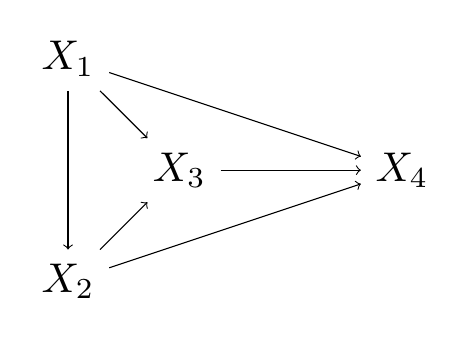
\begin{tikzpicture}[scale=2,rotate=45]
\node[scale=1.5] (X1) at (0,2) {$X_1$};
\node[scale=1.5] (X2) at (-1,1) {$X_2$};
\node[scale=1.5] (X3) at (0,1) {$X_3$};
\node[scale=1.5] (X4) at (1,0) {$X_4$};
\draw[->] (X1) -- (X2);
\draw[->] (X1) -- (X3);
\draw[->] (X1) -- (X4);
\draw[->] (X2) -- (X3);
\draw[->] (X2) -- (X4);
\draw[->] (X3) -- (X4);
\end{tikzpicture}
\end{center}
\end{example}

\begin{example}
Une distribution pour laquelle les variables $X_1,\dots,X_n$ sont indépendants est compatible avec tout DAG sur $V$.
\end{example}

\begin{example}[Exécution]
  \label{ex:dag-execution}
Le graphe de l'exemple de l'Exécution Section~\ref{sec:exemple-intr-i} se résume à $X\to Y$, il s'agit bien d'un DAG. C'est un cas particulier de l'exemple~\ref{ex:dag-maximal}. $G$ est donc Markov-compatible avec toute distribution jointe pour $(X,Y)$. 
\end{example}

\begin{example}[Sol mouillé]
Dans l'exemple du Sol moullié Section~\ref{sec:exemple-intr-ii}, les flèches dessinées définissent bien un DAG $G$ sur $V=(X_1,\dots,X_4)$. De plus, montrons que la distribution $P$ considérée est Markov-compatible avec $G$.
La variable $X_4$ étant par définition une fonction déterministe de
$X_2$ et de $X_3$, et puisque d'après le graphe dessiné on a
$PA_4=(X_2,X_3)$, on peut écrire:
\[ P(x_4|x_1,x_2,x_3)=P(x_4|x_2,x_3)=P(x_4|pa_4). \]
De même, $X_3$ étant une fonction déterministe de $X_1$, et puisque $PA_3=X_1$:
\[ P(x_3|x_1,x_2)=P(x_3|x_1)=P(x_3|pa_3). \]
Puis comme $PA_2=\left\{ X_1 \right\}$:
\[ P(x_2|x_1)=P(x_2|pa_2). \]
Et enfin, $X_1$ n'a pas de parents, donc:
\[ P(x_1)=P(x_1|pa_1). \] Les égalités ci-dessus assurent que
l'identité de la Définition~\ref{def:markov-compatibilite} est
satisfaite.  $P$ et $G$ sont donc bien Markov-compatibles.
\end{example}

La Markov-compatibilité entre un DAG $G$ et une distribution $P$
permet de rendre compte de relations entres les variables aléatoires.
On va à présent considérer une interprétation supplémentaire des DAG:
ils vont servir à représenter également des \emph{liens de
  causalité}. Dans la section suivante, le choix d'un DAG compatible
avec la distribution va permettre de définir comment la distribution
est \emph{modifiée par une intervention}.

\section{La distribution $P(\,\cdot\,|\,do(X=x))$}
\label{sec:la-distribution-p}

\begin{definition}
La donnée de $(V,P,G)$ où
\begin{itemize}
\item $P$ est une distribution pour $V$;
\item $G$ est un DAG sur $V$;
\item $P$ et $G$ sont Markov-compatibles;
\end{itemize}
est appelé \emph{Causal Bayesian Network} (CBN).
\end{definition}


On définit à présent les distributions \emph{modifiées par une intervention}.

\begin{definition}
On note $V=(V_i)_{i\in I}$. Soit 
\begin{itemize}
\item $X=(V_i)_{i\in J}$ et $Y=(V_j)_{i\in K}$ deux sous-ensembles de $V$,
\item $x=(x_i)_{i\in J}\in D_{X}$ et  $y=(y_i)_{i\in K}\in D_Y$.
\end{itemize}
On dit que \og$Y=y$\fg\ (ou \og$y$\fg tout court) est compatible avec \og$X=x$\fg\ (ou $x$ tout court) si:
\[ \forall i\in J\cap K,\quad y_i=x_i. \]
\end{definition}

\begin{proposition}
  \label{prop:Px}
Soit $(V=(V_i)_{i\in I},P,G)$ un CBN, $X\subset V$ un sous-ensemble de variables, et $x\in D_X$ une valeur possible pour $X$.
On considère $P_x$ la fonction de $D_V$ dans $[0,1]$ donnée par:
\begin{equation}
\label{eq:2}
\forall v\in D_{V},\quad P_x(v):=
\begin{cases}
\displaystyle \prod_{\substack{i\in I\\V_i\not \in X}}^{}P(v_i|pa_i)&\text{si $x$ compat. avec $v$}\\
0&\text{sinon}.
\end{cases}
\end{equation}
où $pa_i$ est une abbréviation de: \[ V_j=v_j,\quad \text{pour tout $j$ tel que $V_j\in PA_i$}. \]
Alors $P_x$ définit une distribution de probabilité pour $V$.
\end{proposition}
\begin{proof}
$P_x$ est à valeurs dans $[0,1]$. Il suffit de montrer que:
\[ \sum_{v\in D_V}^{}P_x(v)=1. \]
Pour chaque $i\in I$, considérons l'ensemble
\[ \tilde{D}_{V_i}:=
  \begin{cases}
    D_{V_i}&\text{si $V_i\not \in X$}\\
    \left\{ x_i \right\}&\text{si $V_i\in X$};
  \end{cases}
\]
autrement dit, $\tilde{D}_{V_i}$ est l'ensemble des valeurs possibles de la
variable $V_i$ compatibles avec l'intervention $X=x$. Par ailleurs, pour tout $i\in \mathcal{I}$, $v_i\in D_{V_i}$ et $pa_i\in D_{PA_i}$, on considère la notation:
\[ \tilde{P}(v_i|pa_i):=
\begin{cases}
  P(v_i|pa_i)&\text{si $V_i\not \in X$}\\
  1&\text{si $V_i\in X$}.
\end{cases} \]
On peut alors traduire la truncated factorization comme suit:
\begin{align*}
\sum_{v\in D_V}^{}P_x(v)&=\sum_{v_1\in D_{V_1}}^{}\dots \sum_{v_n\in D_{V_n}}^{}P_x(v)\\
&=\sum_{v_1\in \tilde{D}_{V_1}}^{}\dots \sum_{v_n\in
                    \tilde{D}_{V_n}}^{}P_x(v)\\
&=\sum_{v_1\in \tilde{D}_{V_1}}^{}\dots \sum_{v_n\in \tilde{D}_{V_n}}^{}\prod_{i=1}^n\tilde{P}(v_i|pa_i).
\end{align*}
$G$ étant acyclique, quitte à réindicer les variables, on peut
supposer que $I=\left\{ 1,\dots,n \right\}$ et que $PA_i\subset
(X_1,\dots,X_{i-1})$ pour tout $i\in I$. Cela nous permet de
factoriser l'expression ci-dessus de la façon suivante:
\begin{equation}
\label{eq:1}
\sum_{v\in D_V}^{}P_x(v)=\sum_{v_1\in \tilde{D}_{V_1}}^{}\tilde{P}(v_1)\sum_{v_2\in \tilde{D}_{V_2}}^{}\tilde{P}(v_2|pa_2)\sum_{v_3\in \tilde{D}_{V_3}}^{}\dots \sum_{v_n\in \tilde{D}_{V_n}}^{}\tilde{P}(v_n|pa_n).
\end{equation}
Par ailleurs, on a $\sum_{v_i\in D_{V_i}}^{}\tilde{P}(v_i|pa_i)=1$ pour tout $i\in I$; en effet dans le cas $V_i\in X$, la somme ne contient qu'un seul terme égal à 1, et dans le cas $V_i\not \in X$, $\tilde{P}(v_i|pa_i)=P(v_i|pa_i)$ par définition de $\tilde{P}$ et la somme vaut alors $1$ car $P$ est une distribution de probabilité.
L'équation (\ref{eq:1}) se simplifie donc en:
\[ \sum_{v\in D_V}^{}P_x(v)=1. \]
\end{proof}

L'expression (\ref{eq:2}) est appellée \emph{truncated factorization}.

\begin{definition}
La distribution introduite dans la Proposition~\ref{prop:Px} est appelée \emph{modification de la distribution initiale $P$ par l'intervention $X=x$}.
Elle est notée:
\[ P_x=P_{X=x}=P(\,\cdot\,|do(x))=P(\,\cdot\,|do(X=x)). \]
\end{definition}

\begin{proposition}
Soit $(V=(V_i)_{i\in I},P,G)$ un CBN, $X\subset V$ un sous-ensemble de variables, et $x\in D_X$ une valeur possible pour $X$.
Soit également $V_i\in V$ une variable, $v_i\in D_{V_i}$, $pa_i\in D_{PA_i}$.
La distribution $P_x$ satisfait les propriétés suivantes.
\begin{enumerate}[(i)]
\item\label{item:1} $P_x$ est Markov-compatible avec $G$.
\item\label{item:2} Si $V_i\in X$ et $v_i$ compatible avec $X=x$, alors $P_x(v_i)=1$.
\item\label{item:3} Si $V_i\not \in X$ et $pa_i$ compatible avec $X=x$, alors $P_x(v_i|pa_i)=P(v_i|pa_i)$.
\item $P(v_i|pa_i)=P_{pa_i}(v_i)$,
\item Si $S\subset V\setminus (\left\{ V_i \right\}\cup PA_i)$ et $s\in D_S$, alors $P_{pa_i,s}(v_i)=P_{pa_i}(v_i)$.
\end{enumerate} 
\end{proposition}

\begin{remark}
La \emph{truncated factorization} permet d'estimer l'effet d'une intervention à partir de données tirées selon la distribution initiale $P$, c'est-à-dire \emph{sans faire d'intervention}.
\end{remark}

\begin{example}[Exécution]
On considère à nouveau l'exemple de la Section~\ref{sec:exemple-intr-i}.
Calculons la probabilité pour le condamné de mourir ($Y=1$) lorsqu'on \emph{intervient pour forcer} le tireur à tirer ($X=1$). On écrit d'abord:
\[ P_{X=1}(Y=1)=P_{X=1}(X=0,Y=1)+P_{X=1}(X=1,Y=1). \]
Le premier terme du membre de droite est nul, car la configuration $(X=0,Y=1)$ n'est pas compatible avec l'intervention $X=1$. 
On exprime le second terme à l'aide de la \emph{truncated factorization}:
\[ P_{X=1}(X=1,Y=1)=P(Y=1|PA_Y=1)=P(Y=1|X=1)=1, \]
où la deuxième égalité découle simplement du fait que $X$ est le seul parent de $Y$.
On a donc $P_{X=1}(Y=1)=1$, ce qui est bien la réponse à laquelle on s'attendait.

Calculons à présent la probabilité pour le tireur de tirer ($X=1$) lorsqu'on \emph{intervient pour forcer} la mort du condamné ($Y=1$):
\begin{align*}
P_{Y=1}(X=1)&=P_{Y=1}(X=1,Y=0)+P_{Y=1}(X=1,Y=1)\\
&=P_{Y=1}(X=1,Y=1)\\
&=P(X=1|PA_X)\\
&=P(X=1)=\frac{1}{2},
\end{align*}
où la troisèmé égalité écoule de la truncated factorization, et la quatrième égalité du fait que $X$ n'a pas de parent dans le DAG considéré. Il s'agit bien de la réponse attendue.

On peut voir sur cet exemple que le choix du DAG $G$ (parmi tous les DAG Markov-compatibles avec la distribution $P$) 
détermine de façon cruciale la distribution modifiée par une intervention. Les quantités calculées ci-dessus auraient eu leurs valeurs permutées si on avait considéré le DAG $Y\to X$, qui est lui aussi Markov-compatible avec $P$ (comme on l'a vu dans l'Exemple~\ref{ex:dag-execution}). 
\end{example}

%%% Local Variables:
%%% mode: latex
%%% TeX-master: "../causality-notes"
%%% End:
